% -------------------------------------- Workflows and Tools ----------------------------------
\clearpage
\section{Workflows and Tools}

% Generate Hierarchy 
\subsection{Generate Hierarchy}

% ReadOBJ
\subsection{ReadOBJ}

% Combining Geometries
\subsection{Combining Geometries}

% SRAGCodes
\subsection{SRAGCodes}
The \texttt{SRAGCodes} repository is a software library that allows sampling of Galactic Cosmic Ray (GCR)
spectra for any Monte Carlo code. The library is written with C++ interfaces and coded using the C++11 
standard. The repository contains GCR spectra for Badhwar O'Neill 2014 Model (BOM), Local Interstellar Spectrum, and
the 1996 BOM model.

\subsubsection*{Build SRAGCodes}
To build the SRAGCodes repository, first clone the git repository from https://github.com/kerrylee01/SRAGCodes.git
\lstset{language=bash} 
\begin{lstlisting}
cd SRAGCodes
mkdir bld
cd bld
cmake .. -DCMAKE_INSTALL_PREFIX=..
make -j
make install
make test
\end{lstlisting}
The above listing shows the full install procedure including the running of the installation tests. In order to build
Fluka with the SRAGCodes linked in run the build\_fluka script found in the base directory of the SRAGCodes repository.
\subsubsection*{Running Fluka with SRAGCodes}
First, you must set the GCR\_SOURCE\_PATH environment variable to tell the Fluka executable where to find the GCR data. 
\begin{lstlisting}
export GCR_SOURCE_PATH=/path/to/SRAGCodes/RadSource/GCRSource/
\end{lstlisting}
In the Fluka input you wish to run you must add the source decription, there are currently two main types of 
geometric sampling, Spherical Element where you specify a target area and source radius and Sphere where an isotropic
inward directed. The geometry of the spherical element source is shown in Figure \ref{fig:spherical_element}.

\begin{figure}[ht!]
 \begin{centering}
 \centering
 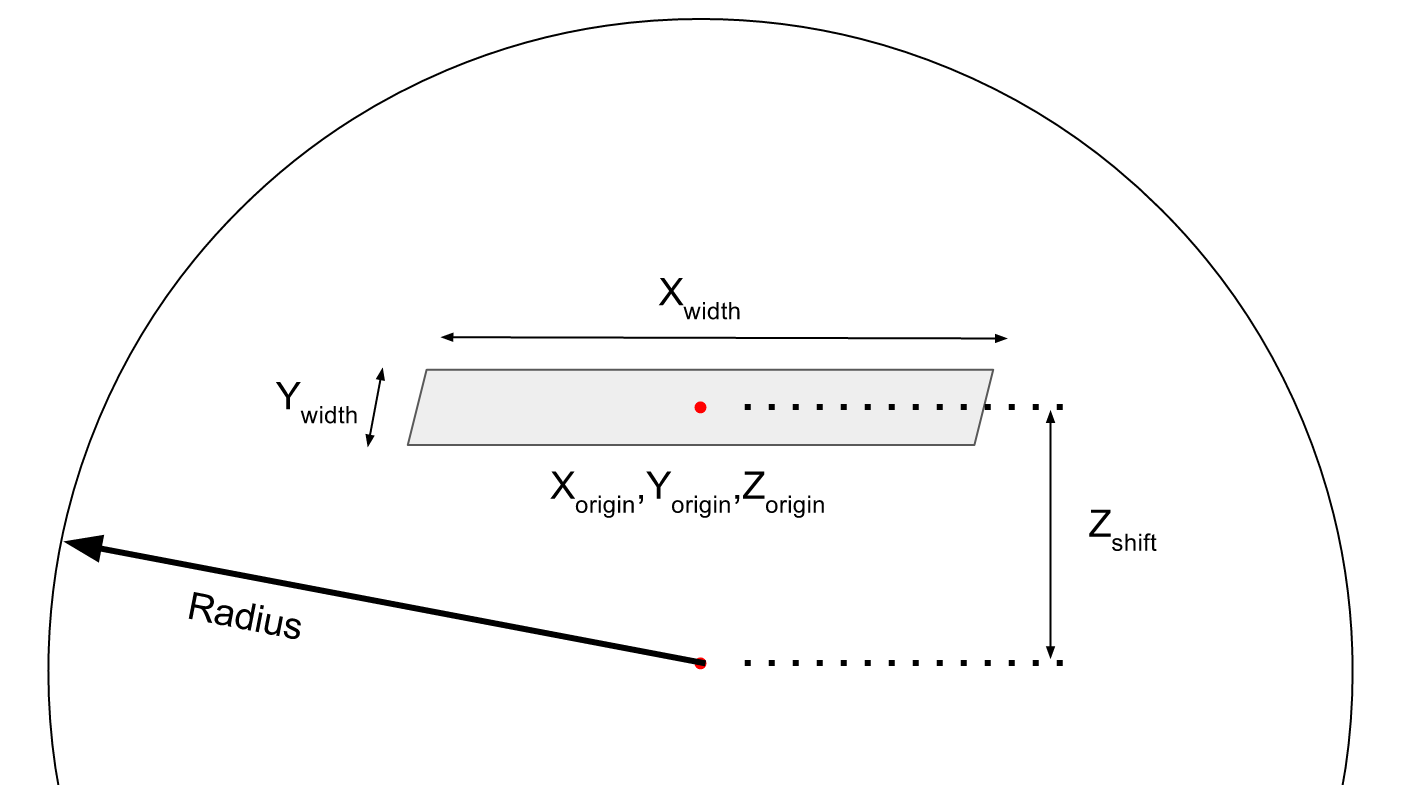
\includegraphics[width=0.6\paperwidth]{../figs/spherical_element_source.png}
 \caption{Geometry of the input parameters for the Spherical Element source}
 \label{fig:spherical_element}
 \end{centering}
\end{figure}
Please note that the vertical shift is relative to the origin, so negative values mean the sphere origin is moved below the target plane
and positive values are above the source plane. Source particles are sampled by picking a random x,y coordinate in the range of the 
widths, a ray direction is istropically sampled in the positive z direction, and this ray is then intersected with the sampling sphere, 
this intersection point marks the start x,y,z coordinate of the source particle, the direction is similarly defined. The particle weight
is then set based on the solid angle of the target area from the intersection point, which effectively defines the probability of 
any source particle at this point intersecting with the target area. Please note that since particles are traced back from the target 
rectangle to the source sphere, particles are therefore sampled such that particles are born only above the visible horizon.  

\begin{table}[ht!]
 \begin{tabular}{c|c}
 Entry & Value \\
 \hline
 SDUM & SPHELE \\
 WHASOU(1) & X Origin (cm) \\
 WHASOU(2) & Y Origin (cm) \\
 WHASOU(3) & Z Origin (cm) \\
 WHASOU(4) & X Width  (cm) \\
 WHASOU(5) & Y Width  (cm) \\
 WHASOU(6) & Radius   (cm) \\
 WHASOU(7) & Z Shift  (cm) \\
 WHASOU(8) & Particle ID to sample \\
 WHASOU(9) & Source Type 
 \end{tabular}
\label{tab:sphele_source}
\caption{Source sampling options for the Spherical Element Source}
\end{table}

\begin{table}[ht!]
 \begin{tabular}{c|c}
 Entry & Value \\
 \hline
 SDUM & SPHERE \\
 WHASOU(1) & Radius (cm) \\
 WHASOU(8) & Particle ID to sample \\
 WHASOU(9) & Source Type 
 \end{tabular}
\label{tab:sphere_source}
\caption{Source sampling options for the Spherical source}
\end{table}

\subsubsection*{Particle ID}
Both of the source sampling methods require the entry of the particle id to sample,
\begin{table}[ht!]
 \begin{tabular}{c|c}
 Entry & Result \\
 \hline
 0  & sample all particles according to PDF \\
 1  & hydrogen isotopes only \\
 2  & helium isotopes only \\
 ... & ... \\
 28 & nickel isotopes only \\
 \end{tabular}
\label{tab:particleid}
\caption{Source sampling options for the Spherical source}
\end{table}

\subsubsection*{Source Type}
Both of the source sampling methods require the entry of the source type to sample
\begin{table}[ht!]
 \begin{tabular}{c|c}
 Entry & Result \\
 \hline
 0  & BOM Jan 2003 \\
 1  & BOM 2014 from 11/15/2015 to 1/15/2016 \\
 2  & BOM 2014 \\
 \end{tabular}
\label{tab:source_type}
\caption{Source sampling options for the Spherical source}
\end{table}

\subsubsection*{Source Sampling}
The main C++ layers of the SRAGCodes library is hideen behind a C safe callable routine that can be linked
against C/C++ and Fortran codes. The two functions exposed are \texttt{setup()} and \texttt{sample()}. 
\subsubsection*{setup}
The setup function is nessessarily long as we have to pass simple inputs to more complex C++ structures
in the SRAGCodes layer.
\lstset{language=C++}
\begin{lstlisting}
void setup_(double &origin_x, double &origin_y, double &origin_z,
        double &x_width, double &y_width, double &radius,
        double &z_shift, int &ionid, int &spectrum_type, int &error,
        char* src_type, int &string_length)
\end{lstlisting}

\subsubsection*{sample}
\begin{lstlisting}
void sample_source_(double *randoms, int& num_randoms, double &xxx, 
        double &yyy, double &zzz, double &uuu, 
        double &vvv, double &www, double &energy, 
        double &weight, double &atomic_mass,
        int &ionID, int &charge, int &nucleon_num)
\end{lstlisting}
There are two main ways of sampling from the source routine, either pass in a populated vector
of uniformly distributed random numbers e.g. \texttt{double array[6];} or 
\texttt{double precision array(6)} and set the \texttt{num\_randoms} variable to 6, or you 
can use the internal C++11 random number generator by passing an array and setting
\texttt{num\_randoms} to 1. The source routine will then return to you 
an appropriately distributed particle start coordinate \texttt{xxx},\texttt{yyy},\texttt{zzz} and
noramlised direction vectors \texttt{uuu},\texttt{vvv},\texttt{www}. The energy returned
in the \texttt{energy} variable is in GeV, the statistical weight \texttt{weight} is a weight
between 0 and 1. The ionId variable is Fluka specific and lets fluka know if it is a heavy
ion or not, in Fluka heavy ions are defined as particles with greater atomic number than 2. 
The atomic mass, charge and nucleon number serve to uniquely indentify the particle returned 
from the sampling routine. 



